\lab{Applications}{Hysteresis}{Bifurcations}
\label{lab:Bifurcations}

Recall that any ordinary differential equation can be written as a first order system of DEs, 
\begin{align}
\dot{x} = F(x), \quad \dot{x} := \frac{d}{dt}x(t).\label{fos}
\end{align}
Many interesting applications and physical phenemena can be modelled using ODEs.  Given a mathematical model of the form \eqref{fos}, it is important to understand geometrically how its solutions behave.  This information can then be conveyed in a phase portrait, a graph describing solutions of \eqref{fos} with differential initial conditions.  The first step in constructing a phase portrait is to find the equilibrium solutions of the equation, i.e., the zeros of $F(x)$, and to determine their stability. 

It is often the case that the mathematical model we study depends on some parameter or set of parameters $\lambda$.  Thus the ODE becomes 
\begin{align}
\dot{x} = F(x,\lambda).\label{fos2}
\end{align}
The parameter $\lambda$ can then be tuned to better fit the physical application.  As $\lambda$ varies, the equilibrium solutions and other geometric features of \eqref{fos2} may suddenly change.  A value of $\lambda$ where the phase portrait changes is called a \emph{bifurcation point}; the study of how these changes occur is called \emph{bifurcation theory}.  The parameter values and corresponding equilibrium solutions are often graphed together in a bifurcation diagram. 

As an example, consider the scalar differential equation 
\begin{eqnarray}
\dot{x} &=& x^2 + \lambda. \label{snbifurcation}
\end{eqnarray}
For $\lambda > 0$ equation (\ref{snbifurcation}) has no equilibrium solutions.  At $\lambda = 0$ the equilibrium point $x=0$ appears, and for $\lambda < 0$ it splits into two equilibrium points.  For this system, a bifurcation occurs at $\lambda = 0$.  This is an example of a saddle-node bifurcation.  The bifurcation diagram is shown in Figure \ref{bifurcation:sn} 


\begin{figure}[ht]
\centering
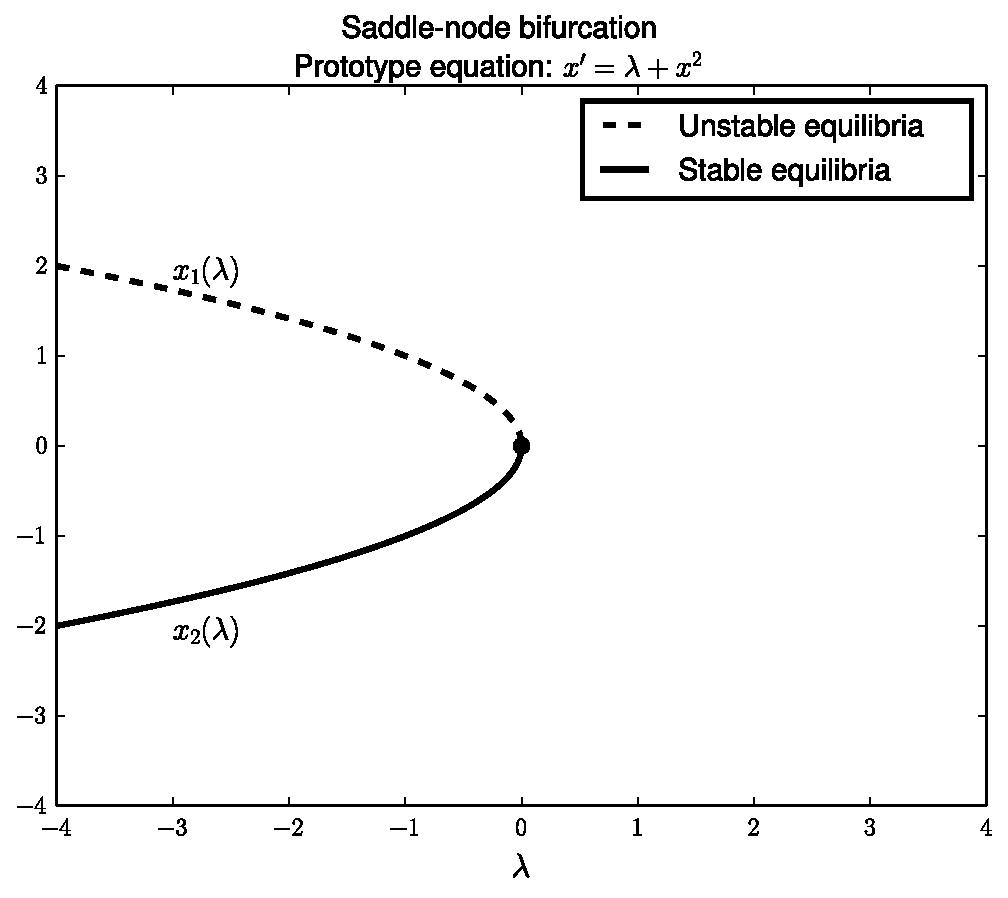
\includegraphics[width=\textwidth]{SaddleNBifurcation.pdf}
\caption{Bifurcation diagram for the equation $\dot{x} = \lambda + x^2$.}
\label{bifurcation:sn}
\end{figure}

\begin{figure}[ht]
\centering
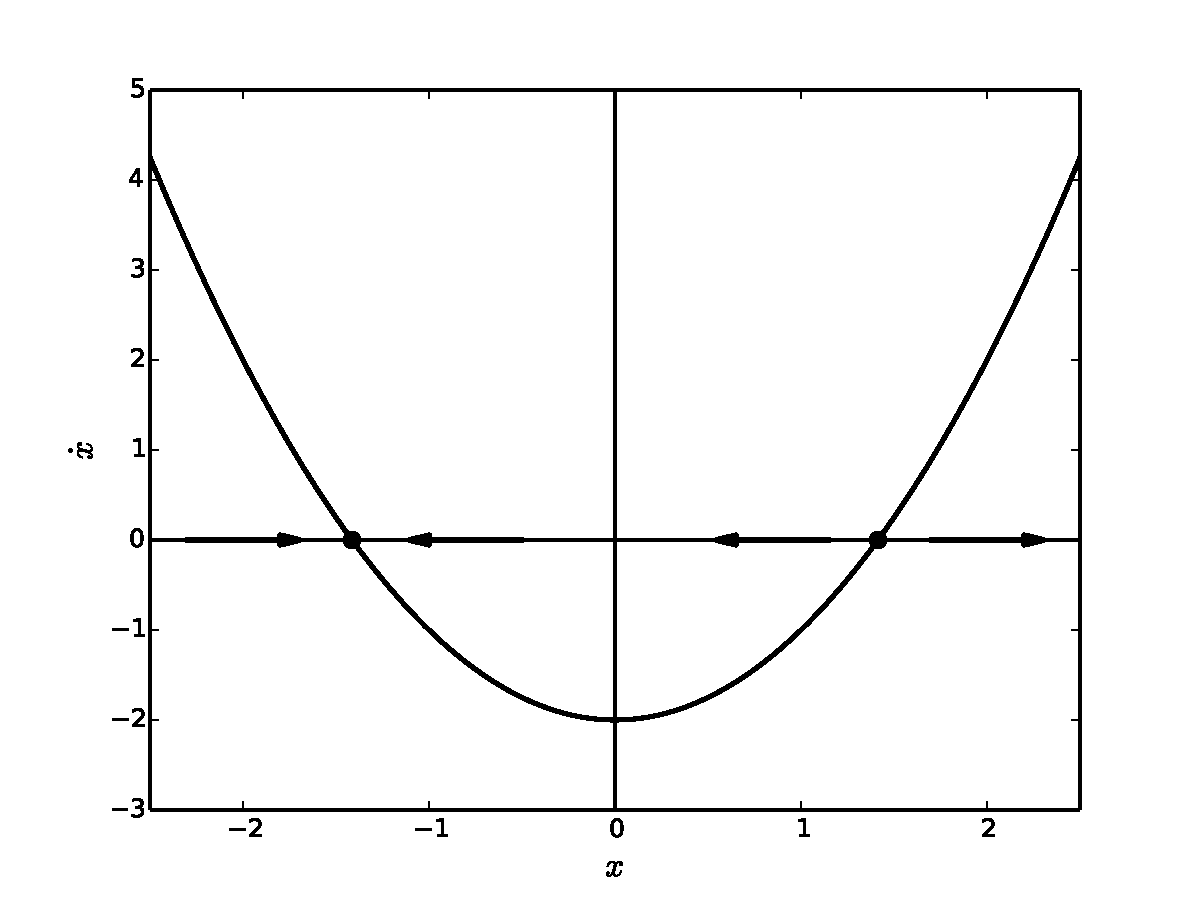
\includegraphics[width=\textwidth]{SaddleNPhasePortrait.pdf}
\caption{Phase Portrait for the equation $\dot{x} = -2 + x^2$.}
\label{phaseportrait:sn}
\end{figure}

% The flow of a differential equation \[\dot{x} = f(x)\] is the family of all possible solutions $\phi(t,x_0)$, where $x_0$ represents the arbitrary initial value, $t \in \mathbb{R}.$ Here we will mainly consider scalar differential equations (so-called because $x$ is one dimensional). It is often necessary to study a family of differential equations. These will have the form 
% \[\dot{x}= F(x,c),\]
% where $c$ may be a single parameter or a vector of parameters. 
% 
% Bifurcation theory is the study of how the qualitative structure of the flow of a differential equation varies as parameters in the differential equation are varied. 
% A differential equation has a stable orbit structure if sufficiently small changes in the parameter value do not change the qualitative structure of the flow.
% A parameter value for which the flow does not have a stable orbit structure is called a bifurcation value.
% 
% Terminology
% bifurcation theory: 'the study of possible changes in the structure of orbits of a differential equation depending on variable parameters'
% 'the study of changes in the qualitative structure of the flow of a differential equation as parameters are varied'
% phase portrait: 
% bifurcation diagram: 
% number of orbits and their direction of flow of a differential equation = 'orbit structure of the differential equation' or 'the qualitiative structure of the flow'.
%  
% 
% Hyperbolic equilibrium points
% $F(x_0,c_0) = 0$ where $\frac{df}{dx}(x_0,c_0) \not = 0.$ In this case the stability of the equilibrium point $x_0$ for values of $c$ near $c_0$ is determined by the derivative $\frac{df}{dx}(x_0,c_0)$.
% Example: $\dot{x} = x-c.$ Plot $x$
% 
% Hyperbolic equilibrium - mainly to be used when discussing stability
% Saddle-Node Bifurcation - \[\dot{x} = c + x^2.\]
% Transcritical Bifurcation - \[\dot{x} = cx + x^2.\]
% Hysteresis Loop - \[\dot{x} = c + x-x^3.\]
% Pitchfork Bifurcation (Supercritical) - \[\dot{x} = cx-x^3.\]
% For an exercise, do a variation of \[\dot{x} = 1+cx-x^3.\]
% 


Suppose that $F(x_0,\lambda_0) = 0.$  We use a method called natural embedding to find zeros $(x,\lambda)$ of $F$ for nearby values of $\lambda$.  Specifically, we step forward in $\lambda$ by letting $\lambda_1 = \lambda_0 + \triangle \lambda$, and use Newton's method to find the value $x_1$ that satisfies $F(x_1,\lambda_1) = 0.$  This method works well except when $\lambda$ is near a bifurcation point $\lambda^*$.

The following code implements the natural embedding algorithm, and then uses that algorithm to find the curves in the bifurcation diagram for (\ref{snbifurcation}).  Notice that this algorithm needs a good initial guess for $x_0$ to get started. 

\begin{lstlisting}
import numpy as np
import matplotlib.pyplot as plt
from scipy.optimize import newton

def EmbeddingAlg(param_list,guess,F):
	X = []
	for param in param_list:
		try:
			# Fix the parameter value inside the function.
			g = lambda x, param=param: F(x,param)
			# Solve for x_value making F(x_value, param) = 0.
			x_value = newton(g, guess, fprime=None, 
								args=(), tol=1.0e-08, maxiter=50)
			
			# Record the solution and update guess for 
			# the next iteration
			X.append(x_value)
			guess = x_value 
		except:
			return param_list[:len(X)], X	
	return param_list[:len(X)], X   		
	# returns the (possibly truncated) list of parameter values 
	# and corresponding x values


def F(x,lmbda):
	return x**2. + lmbda

# Top curve shown in the bifurcation diagram
C1, X1 = EmbeddingAlg(np.linspace(-5,0,200),np.sqrt(5),F)
# The bottom curve
C2, X2 = EmbeddingAlg(np.linspace(-5,0,200),-np.sqrt(5),F)
\end{lstlisting}


\begin{problem}
Use the natural embedding algorithm to create a bifurcation diagram for the differential equation
\[\dot{x} = \lambda x-x^3.\]
This type of bifurcation is called a pitchfork bifurcation (you should see a pitchfork in your diagram).
\end{problem}

\begin{problem}
Create bifurcation diagrams for the differential equation
\[\dot{x} = \eta + \lambda x-x^3,\]
where $\eta = -1, -.2, .2$ and $1.$  Notice that when $\eta = 0$ you can see the pitchfork bifurcation of the previous problem.
\end{problem}

An interesting ODE is given by 
\begin{align*}
	x' &= \lambda + x - x^3.
\end{align*}
This system has a bifurcation diagram containing what is known as a hysteresis loop, shown in Figure \ref{bifurcation:hysteresis}.  In the hysteresis loop, when the parameter $\lambda$ moves beyond the bifurcation point the equilibrium solution makes a sudden jump to the other stable branch.  When this occurs the system cannot reach its previous equilibrium by simply rewinding the parameter slightly. 


\begin{figure}[ht]
\centering
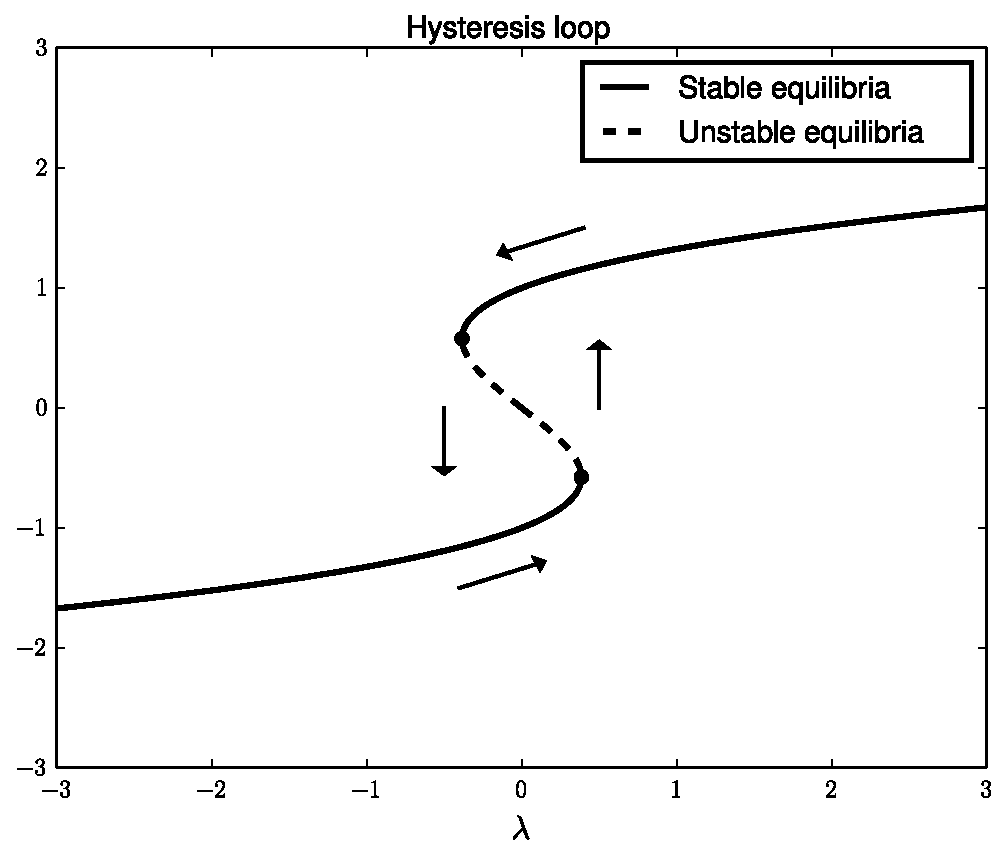
\includegraphics[width=\textwidth]{HysteresisBifurcation.pdf}
\caption{Bifurcation diagram for the ODE $x' = \lambda + x - x^3$. }
\label{bifurcation:hysteresis}
\end{figure}


\section{Budworm Population Dynamics}
Here we study a mathematical model describing the population dynamics of an insect called the spruce budworm. In eastern Canada, an outbreak in the budworm population can destroy a most of the trees in a forest of balsam fir trees in about 4 years.  The mathematical model is given by 
\begin{align}
\dot{N} = RN\left(1 - \frac{N}{K}\right) - p(N). \label{budworm1}
\end{align}
This model was studied by Ludwig et al (1978), and is described well in Strogatz's text \emph{Nonlinear Dynamics and Chaos}.  Here $N(t)$ represents the budworm population at time $t$, $R$ is the growth rate of the budworm population and $K$ represents the carrying capacity of the environment.  We could interpret $K$ to represent the amount of food available to the budworms. 
$p(N)$ represents the death rate of budworms due to predators (birds); we assume specifically that $p(N)$ has the form $P(N) = \frac{BN^2}{A^2 + N^2}$.

Before studying the equilibrium points of \eqref{budworm1} it is important to reduce the number of parameters in the system by nondimensionalizing.  Thus, we make the coordinate change $x = N/A$, $\tau = Bt/A$, $r = RA/B$, and $k = K/A$, obtaining finally the system 
\begin{align}
	\frac{dx}{d \tau} &= rx(1-x/k) - \frac{x^2}{1+x^2}.
\end{align}


Note that $x = 0$ is always an equilibrium solution.  To find other equilibrium solutions we study the equation $r(1-x/k)-x/(1+x^2) = 0$.  Fix $r = .56$, and consider Figure \eqref{equilibria:budworm}. 

\begin{figure}[ht]
\centering
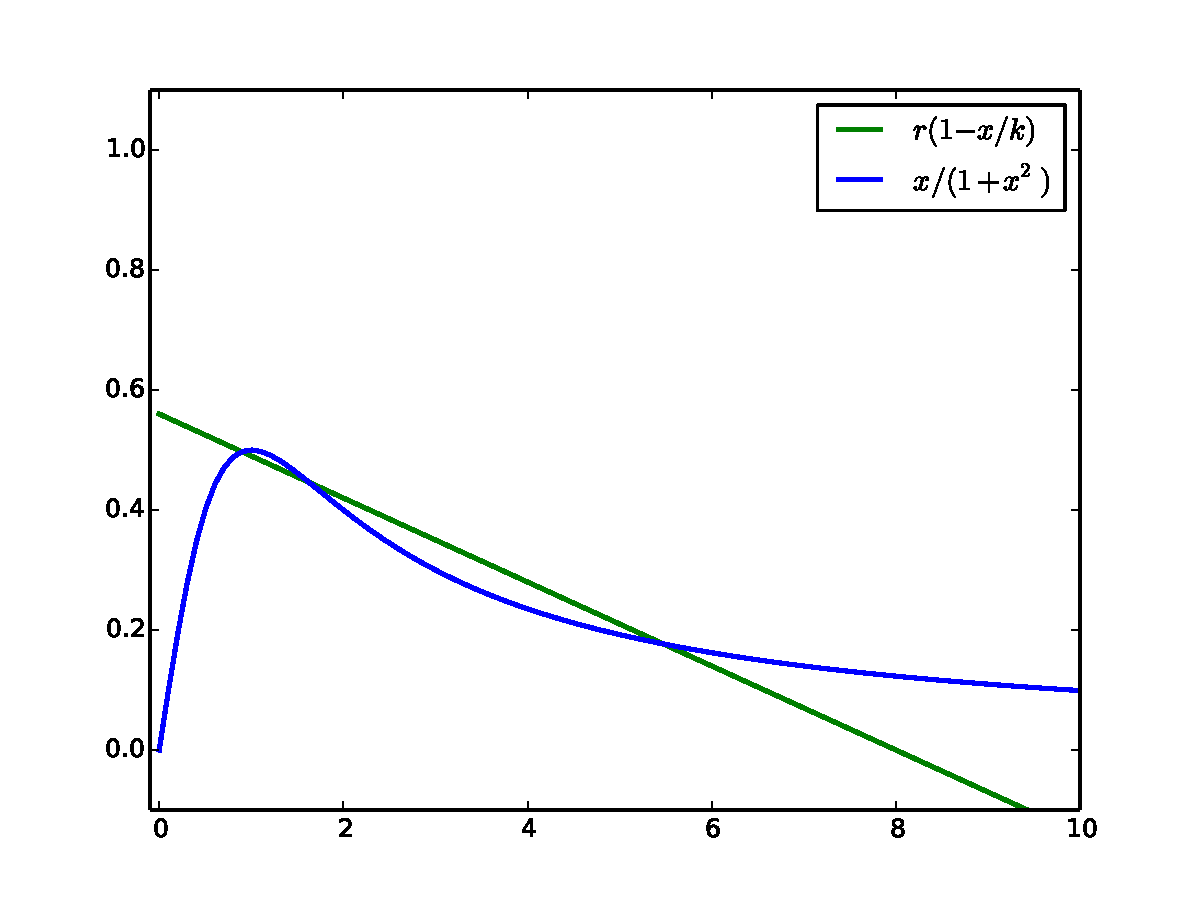
\includegraphics[width=\textwidth]{BudwormEquilibria.pdf}
\caption{Graphical demonstration of nonzero equilibrium solutions for the budworm population (here $r = .56$). Note that as $k$ increases, the number of solutions goes from one to three, and then back to one. }
\label{equilibria:budworm}
\end{figure}

\begin{figure}[ht]
\centering
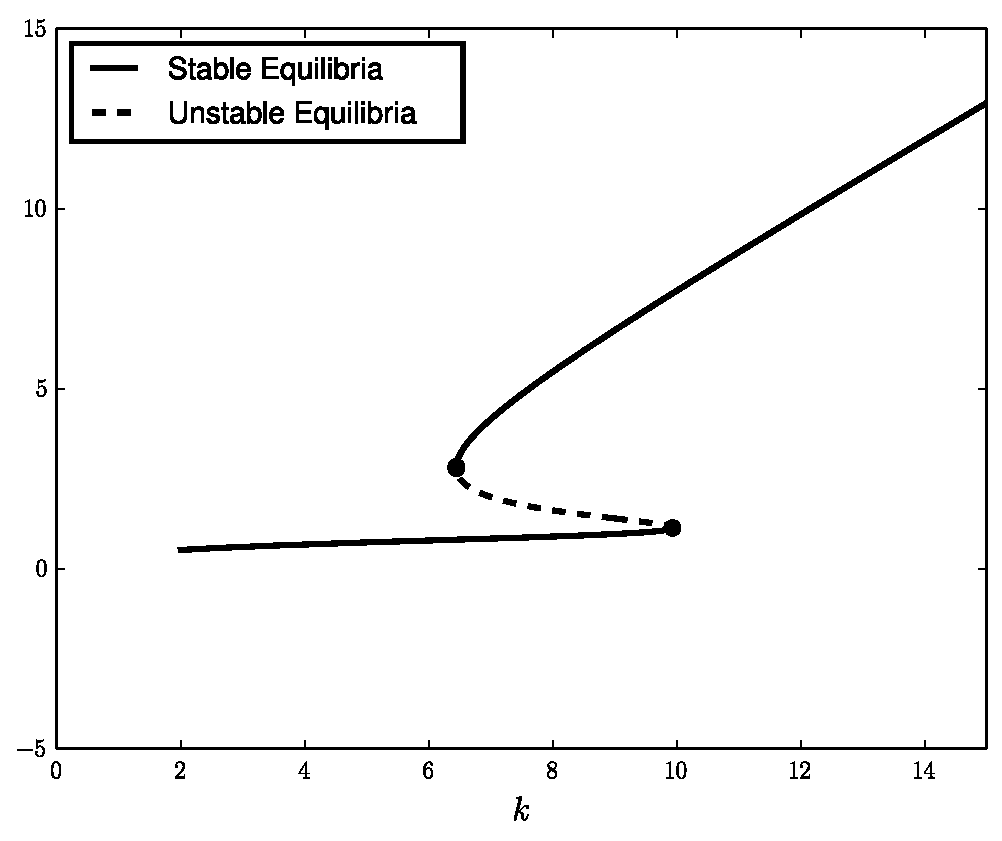
\includegraphics[width=\textwidth]{BudwormPopulation.pdf}
\caption{Bifurcation diagram for the budworm population model. The parameter $r$ is fixed at $0.56.$ The lower stable branch is known as the refuge level of the bundworm population, while the upper stable branch is known as the outbreak level. Once the budworm population is reaches an outbreak level, the available food (foliage of the balsam fir trees) in the system must be reduced drastically to jump back down to refuge level.  Thus many of the balsam fir trees die before the budworm population returns to refuge level.}
\label{bifurcation:budworm}
\end{figure}





\begin{problem}[Budworm Population]
Reproduce the bifurcation diagram for the differential equation
\begin{align*}
	\frac{dx}{d \tau} &= rx(1-x/k) - \frac{x^2}{1+x^2},
\end{align*}
where $r = 0.56$.
\end{problem}






